%!TEX root = ../../root.tex

Principal component analysis is a technique of (linear) dimensionality reduction. 

Given some points in a $d$-dimensional space, we are interested in identifying the direction(s) where data changes the most, to neglect the ones where data changes the least. The motivation is, if most datapoints from a distribution share very similar coordinates along a direction (are very close), then neglecting this direction when representing the distribution should not result in a great loss of information content.

In particular, we want to find the $k \leq d$ \emph{orthogonal} directions with the most \emph{variance}. These will form the \emph{basis} (hence the reason we prefer the set of directions to be orthogonal) of a $k$-dimensional subspace of the original $d$-dimensional space of the data, in which we will \emph{project} the datapoints. 

\textbf{Example.} In the plane we have $d = 2$, and we might be interested in the single principal component $k = 1$, and that would be the only dimension later used to represent the data.
\begin{figure}[H]
	\centering
	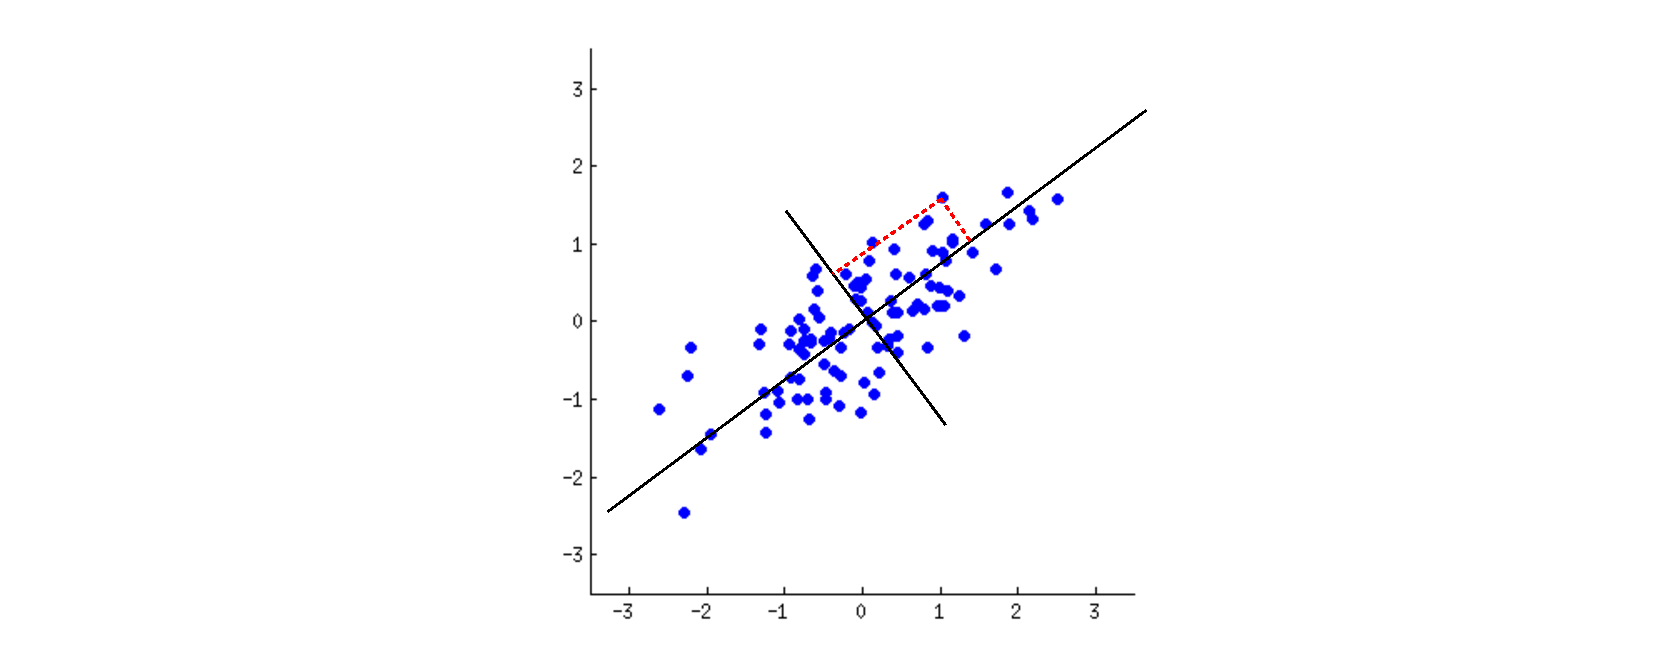
\includegraphics[width=\textwidth]{11/pca3}
	\caption{An example of PCA.}\label{fig:pca-2d}	
\end{figure}

But what do we mean by projection? Suppose we have identified the $k$ principal directions (we will see how to do that later), how do we express a datapoint $\vb{x}$ in terms of these directions?
For each direction, the component of $\vb{x}$ wrt to that direction will be the distance from the origin of the \emph{projection} of the point on the direction. This means that to compute the transformed datapoint $\vb{z}$ we have to compute $k$ dot products between $\vb{x}$ and the $k$-th principal component vector $\vb{w}_k$ (a $d$-dimensional unit vector). This means that this transformation can be encoded by a matrix:
\begin{equation}
	\vb{Z}^{\top} = \underbrace{\left( \begin{smallmatrix}-&\mathbf{z}_1^\top&-  \\ & \vdots & \\ -&\mathbf{z}_n^\top &-\end{smallmatrix} \right)}_{n \times k} =  \underbrace{\left( \begin{smallmatrix}-&\mathbf{x}_1^\top&-  \\ & \vdots & \\ -&\mathbf{x}_n^\top &-\end{smallmatrix} \right)}_{n \times d} \underbrace{\left( \begin{smallmatrix} |& &|\\\mathbf{w}_1& \dots&\mathbf{w}_k \\ |& &| \end{smallmatrix} \right)}_{d \times k} = \vb{X}^{\top} \vb{W} .
\end{equation}


Since PCA assumes that the principal components are orthogonal, if $k = d$ we will have an \emph{orthogonal matrix}:
\begin{equation}
    \vb{W}^{\top} \vb{W} = \vb{I}_{k \times k} = \vb{I}_{d \times d} = \vb{W} \vb{W}^{\top}.
\end{equation}
(see \cref{cl:orthogonal}.)

This implies that for $k = d$ we have
\begin{align}
    \vb{X}^{\top} \vb{W} &= \vb{Z}^{\top} \\
    \vb{X}^{\top} \vb{W} \vb{W}^{\top} &= \vb{Z}^{\top} \vb{W}^{\top} \\
    \vb{X}^{\top} \vb{I}_{d \times d} &= \vb{Z}^{\top} \vb{W}^{\top} \\
    (\vb{X}^{\top})^{\top} &= (\vb{Z}^{\top} \vb{W}^{\top})^{\top} \\
    \vb{X} &= \vb{W} \vb{Z}.
\end{align}
However, we want $k < d$, but in this case the matrix $\vb{W}$ will be only \emph{semi-orthogonal}, since it is non-square. This means that it is 
\begin{equation}
    \vb{W}^{\top} \vb{W} = \vb{I}_{k \times k}, \qquad \vb{W} \vb{W}^{\top} \neq \vb{I}_{d \times d},
\end{equation}
and hence
\begin{equation}
    \begin{aligned}
        \vb{X}^{\top} \vb{W} & = \vb{Z}^{\top} \\
        \vb{X}^{\top} \underbrace{\vb{W} \vb{W}^{\top}}_{\neq \vb{I}_{d \times d}} & = \vb{Z}^{\top} \vb{W}^{\top} \\
        & \vdots \\
        \vb{X} & \approx \vb{W} \vb{Z}.
    \end{aligned}
\end{equation}
So in the general case we have an exact \emph{projection} transformation and an \emph{approximate} reconstruction transformation
\begin{align}
	\mathbf{X}^\top \mathbf{W} &= \mathbf{Z}^\top \label{eq:projection}\\
	\mathbf{X} &\approx \mathbf{W}\mathbf{Z} \label{eq:reconstruction}
\end{align}
and from the lower representation $\mathbf{Z}$ recovering the full rank representation of the data is something that we cannot do in general. 

We have seen that once the directions are set, the transformation is completely determined, so we have to choose an \emph{optimal} set of principal components, wrt to some \emph{criterion}. We want the projection in the lower-dimensional space to be as \emph{lossless} as possible, or dually we want the reconstruction to be as accurate as possible.

So, our criterion to choose the set of principal components will be to minimize the reconstruction error (also called \emph{projection error})
\begin{equation}
    \epsilon = \norm{ \vb{X} - \mathbf{W}\mathbf{Z} }_2^2 = \norm{\vb{X} - \vb{W}\vb{W}^{\top} \vb{X}}_2^2,
\end{equation}
which as it turns out is equivalent to maximizing the variance of the projected data, that recall was the requirement we started with.

\begin{figure}[H]
    \centering
    \animategraphics[loop, autoplay, width=0.7\textwidth]{20}{11/pca/frame}{0}{178}
    \caption{The direction along which the projection error is minimized is also the one over which variance is maximized.}
\end{figure}

Let's consider only one principal component $\vb{w}$ and, to simplify the calculations, let's assume that the data points $\vb{X}$ have zero mean, meaning that they are \emph{centered} at zero. The projections of all $n$ datapoints onto $\vb{w}$ is $\vb{X}^{\top} \vb{w}$. Now, reminding that the projection error is given by 
\begin{equation}
	\sum_{i} \|\mathbf{x}_i - \left(\mathbf{x}_i^\top \mathbf{w}\right)\mathbf{w}\|^2 = \sum_i (\mathbf{x}_i - \left(\mathbf{x}_i^\top \mathbf{w}\right)\mathbf{w})^\top (\mathbf{x}_i - \left(\mathbf{x}_i^\top \mathbf{w}\right)\mathbf{w}) = \sum_i \| \mathbf{x}_i \|_2^{2} - 2(\mathbf{x}_i^\top \mathbf{w})^2 + (\mathbf{x}_i ^ \top \mathbf{w})^2\| \mathbf{w}\|_2^2
\end{equation}
Now, as $\mathbf{w}$ is orthonormal, $\| \mathbf{w}\| = 1$ and thus we are left with
\begin{align}
	\sum_i \| \mathbf{x}_i \|_2^{2} - 2(\mathbf{x}_i^\top \mathbf{w})^2 + (\mathbf{x}_i ^ \top \mathbf{w})^2 
\end{align}

moreover, since we are maximizing wrt to $\mathbf{w}$, we can ignore the $\mathbf{x}_i$s and just maximize the following expression

\begin{equation}
	- \sum_{i} (\mathbf{x}_i^\top \mathbf{w})^2 = -\norm{\vb{X}^{\top} \vb{\mathbf{w}}}_2^2
\end{equation}

or, equivalently, minimize its additive inverse
\begin{equation}
	\norm{\vb{X}^{\top} \vb{w}}_2^2 = \left( \mathbf{X}^\top \mathbf{w} \right)^\top \left( \mathbf{X}^\top \mathbf{w} \right) = \mathbf{w}^\top \underbrace{\left( \mathbf{X}\mathbf{X}^\top \right)}_{\mathbf{C}} \mathbf{w}
\end{equation}
where $\mathbf{C} \in \mathbb{R}^{d \times d}$ is the symmetric \emph{covariance matrix} of the data. 

So we are looking for the vector $\mathbf{w}$ that minimizes the previous quadratic form, and since we are just interested in the direction we can consider the vector $\mathbf{w}$ as having unit norm. This leads to a \emph{constrained optimization problem}:
\begin{equation}
	\min_{\mathbf{w}} \mathbf{w}^\top \mathbf{C} \mathbf{w} \quad \text{s.t.} \ \|\mathbf{w}\|_2 = 1.
\end{equation}

Constrained optimization problems can generally be solved by means of \emph{Lagrange multipliers}, but for this specific type of problems (minimizing a quadratic form with $\mathbf{C}$ symmetric) we have a theorem that gives us an immediate solution.
The \emph{Courant minmax principle} tells us that the problem is solved \emph{globally} (remember quadratic functions are convex so we have global optimality guarantees) by the first eigenvector of $\mathbf{C}$, which will be the principal component, and the corresponding eigenvalue is equal to the quadratic form.

If we want to find the \emph{second} principal component $\vb{w}_2$, after having solved for the first one:
\begin{equation}
	\mathbf{w}_1 = \argmin_{\mathbf{w}} \mathbf{w}^\top \mathbf{C} \mathbf{w} \quad \text{s.t.} \ \|\mathbf{w}\|_2 = 1
\end{equation}
we define a new constrained optimization problem, identical to the previous one but with the additional constraint enforcing the orthogonality of $\vb{w}_2$ wrt to $\vb{w}_1$:
\begin{equation}
    \begin{aligned}
        \mathbf{w}_2 & = \argmin_{\mathbf{w}} \mathbf{w}^\top \mathbf{C} \mathbf{w} \\
        \text{s.t.} & \begin{cases}
            \ \|\mathbf{w}\|_2 = 1 \\
            \mathbf{w}_1^\top \mathbf{w} = 0
        \end{cases}.
    \end{aligned}
\end{equation}
Again, the Courant minmax theorem comes in handy, since it states the solution to this problem is the \emph{second} eigenvector of $\mathbf{C}$, where the eigenvectors of $\mathbf{C}$ are ordered by increasing eigenvalues. If we iterate this procedure we can find the $k$ principal components, that are thus the first $k \ll d$ eigenvectors of $\mathbf{C}$.
\\

\textbf{Note.} PCA is not linear regression, since with the former we compute the error orthogonally to the principal direction while with the latter we compute the error along each coordinate, as can be seen in the following figure:
\begin{figure}[H]
	\centering
	\begin{subfigure}[t]{0.45\linewidth}
		\centering
		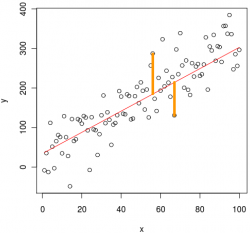
\includegraphics[width=\textwidth]{11/lin1}
		\caption{Linear regression}
	\end{subfigure}
	\hfill
	\begin{subfigure}[t]{0.45\linewidth}
		\centering
		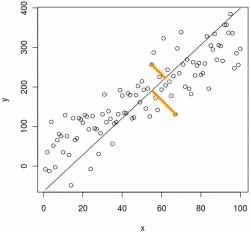
\includegraphics[width=\textwidth]{11/lin2}
		\caption{PCA}
	\end{subfigure}
	\caption{PCA vs Linear regression}
\end{figure}

\paragraph{PCA as a generative model}
PCA can be seen as a generative model. Given the principal components $\mathbf{W}$ we can generate new data just by sampling $\mathbf{z}_{new} \in \mathbb{R}^{k}$ and computing the new sample using reconstruction \cref{eq:reconstruction}:
\begin{equation}
	\mathbf{x}_{new} = \mathbf{W} \mathbf{z}_{new}
\end{equation}

From a different perspective PCA gives us a parametric model. Each data point $\vb{x}$ is transformed into a low-dimensional \emph{code} $\vb{z} \in \mathbb{R}^k$ where the dimension $k < d$ is fixed. The previous relations can be considered as encoding and decoding operations:
\begin{align}
	\mathbf{x}^\top \mathbf{W} &= \mathbf{z}^\top \tag{encoding}\\
	\mathbf{x} &\approx \mathbf{W}\mathbf{z} \tag{decoding}
\end{align}
So passing from the code to the data point is a linear map, specifically a parametric map in which the parameters are the values of matrix $\mathbf{W}$.
For this reason PCA is considered the simplest parametric model since the operation of encoding and decoding are both linear, and we can see this as linear generative model.

A more powerful but complex approach would be to model the encoding and decoding steps as deep neural networks, which grant more control and can be used to enforce the generation of meaningful data, avoiding the generation of gibberish. These, as we know, employ nonlinear transformations instead of linear ones.
